\documentclass{article}
\usepackage{./nips15submit_e,amsmath,amsthm,graphicx,subfig,flafter,tikz}
\usetikzlibrary{shapes,fit}

\newcommand{\eqnref}[1]{equation \eqref{eq:#1}}
\newcommand{\Eqnref}[1]{Equation \eqref{eq:#1}}
\newcommand{\secref}[1]{section \ref{sec:#1}}
\newcommand{\Secref}[1]{Section \ref{sec:#1}}
\newcommand{\thref}[1]{Theorem \ref{th:#1}}
\newcommand{\figref}[1]{figure \ref{fig:#1}}
\newcommand{\Figref}[1]{Figure \ref{fig:#1}}

\newtheorem{theorem}{Theorem}

\title{Attribution Privacy}
\author{
Maxwell Anselm\\
Lehigh University\\
Bethlehem, PA 18015\\
\texttt{mba210@lehigh.edu}\\
}

\nipsfinalcopy
\begin{document}
\maketitle

\section{Introduction}

Peer-to-peer (P2P) networks are a common tool for sharing information. Most P2P
architectures are completely open: the identities of the participants and the
data being shared in the network are available to the public. When privacy is
applied to P2P networks, it is usually done in a way that completely closes down
the network: by making membership in the network invite-only\cite{privatep2p}.

We define a new kind of privacy for P2P networks called ``attribution privacy''
which exists in a traditional open network. Attribution privacy formalizes
the notion that sharing public information among public peers can still leak
private information. We give examples of both real world and technical
applications where attribution privacy is a concern. We also classify when
attribution privacy leaks can occur and measure the potential risk to peers
participating in such a network.

We suggest a couple modifications that can be made to the P2P protocol in order
to mitigate the attribution privacy leaks, and measure their efficacy as well as
their performance impact. We show that these protocol modifications can effectively
protect attribution privacy.

\section{Related Work}\label{sec:relwork}

This work was motivated by our attempt to implement the XRay
system\cite{xray} in a collaborative, P2P environment. XRay audits online
advertisements to reverse-engineer the ad targeting criteria and thus determine
if a company is exploiting one's sensitive information. It does this using a
complicated system of data duplication and fake account management, but the
authors of XRay note that ``a collaborative approach to auditing, in which users
contribute their [data] in a privacy-preserving way is a promising
direction...'' In such a system, users would participate in a P2P network where
they freely share which ads appeared alongside which data in order to help other
peers to determine the actual ad targeting (using differential correlation).
We recognized that sharing such information could potentially leak the private
information that was originally targeted by the ad. Formalizing this type of
privacy leak lead to the definition in \secref{defn}. See \secref{xray} for a
technical description of collaborative XRay as an attribution privacy risk.

We found it necessary to coin the term ``attribution privacy'' after failing to
find similar research in the field of privacy in P2P networks. Most work in this
area appears to focus on protecting the identities of the users involved or
protecting non-participants in the network from seeing what data are being
exchanged\cite{privatep2p}. We suspect that this is due to the strong
association of P2P networks with illegal file-sharing. Although extant private
P2P software would make attribution privacy a moot point (since they ensure that
you can trust the other peers), we show that this level of privacy is
completely independent of attribution privacy.

Because attribution privacy applies to P2P networks, we examined possible P2P
systems to which it might apply. Distributed hash tables (DHT) such as
Chord\cite{chord} appeared to be a possible candidate since they have a notion
of data attribution. However we found that our definition of attribution privacy
does not exactly fit a $(\text{key},\text{value})$ model, but applies in a more
general situation where a value may have fewer or more than 1 key. This fits a
more traditional file-sharing model (e.g. BitTorrent) where data are duplicated
throughout the network as peers demand them.

We also considered other network privacy methods as possible solutions to
attribution privacy leaks. The anonymity provided by Tor
automatically provides attribution privacy as a side-effect (if you do not know
with whom you are communicating, you cannot attribute the data to anyone).
However we show by definition and by example that complete anonymity is not
necessary in situations where attribution privacy is needed. This coupled with
the fact that Tor requires additional infrastructure to function (the relay and
exit nodes) and can significantly impact performance of the network make it a
heavy-handed solution to a much smaller problem. However we do note that one of
our proposed solutions could be extended to a Tor-like protocol for even greater
privacy gains (\secref{future}).

Attribution privacy also bears some similarity with differential privacy: both
are concerned with preserving the utility of the data while protecting the
privacy of the individual. Indeed, differential privacy could even be viewed as
preventing statistical data from being ``attributed'' to an individual. However
these two types of privacy are in actuality very different. Differential
privacy involves a single data set that is queried in aggregate whereas attribution
privacy allows for querying individuals on the network directly. Differential
privacy attempts to ``hide'' individuals among noise in the response whereas
attribution privacy does not allow for modification of the data and only
attempts to hide the data's source. Despite these differences, we do find that a
technique similar to differential privacy's ``randomized
responses''\cite{randresps} works well
for attribution privacy (\secref{unreliable}).

\section{Definitions}\label{sec:defn}

We first define the mechanism and purpose of a P2P network. We imagine a P2P
network in which there are a fixed number of peers (the swarm) and all peers are
aware of the other members of the swarm via some central authority (the
tracker). These peers exchange messages via some secure channel such as HTTPS
(perhaps using public keys synchronised through the tracker). Thus which peers
are communicating with which is public information, while the contents of those
messages is kept private from an observer.

Let $\mathcal{Q}$ be a set of public queries and let $\mathcal{D}$ be a set of
public data about those queries. Imagine the elements of $\mathcal{Q}$ as the
queries that a peer might make to other peers in the swarm, and $\mathcal{D}$ as
potential responses to those queries. Then we define a function
$K:\mathcal{Q}\rightarrow 2^\mathcal{D}$ which maps queries to the set of
possible responses to each query i.e. $\forall q\in\mathcal{Q},
K(q)\subseteq\mathcal{D}$. The reason why peers participate in the network is to
learn more about the ``knowledge function'' $K$. For example, we can imagine
$\mathcal{Q}$ as a set of file names and $\mathcal{D}$ as a set of file
fragments; then $K$ indicates which fragments correspond to which file names
(and which are reused across multiple file names), so determining the value of
$K(q)$ amounts to downloading file $q$. Formally, a response
$D\subseteq\mathcal{D}$ to a query $q\in\mathcal{Q}$ indicates that $D\subseteq
K(q)$. Although peers in the network may not yet know about $K$, we consider $K$
to be public information in the sense that information about $K$ is shared
freely with any peer that requests it.

Next we define $\mathcal{S}$ to be the set of original sources of knowledge
about $K$ in the network. If a peer possesses some source $s\in\mathcal{S}$,
then they can receive some information $D_s\subseteq K(q_s)$ {\it without}
querying another peer in the network. In this case we say that the peer {\it
originates} (or is the {\it origin} of) $D_s\subseteq K(q_s)$. We assume that
the network is otherwise closed, so if a peer wants to learn about $K(q)$ for
some $q$, there need to be peers in the network with sources pertaining to $q$.

For attribution privacy to come into play we need two conditions to hold:
\begin{enumerate}
	\item The sources must be private. That is, a peer with access to some
		$s\in\mathcal{S}$ does not want it to be known publicly.
	\item The relationship between $D_s\subseteq K(q_s)$ and $s\in\mathcal{S}$
		must be public. That is, a peer who sees the response $D\subseteq K(q)$
		will know which sources in $\mathcal{S}$ it might have originated from.
\end{enumerate}

If these conditions hold, then it is possible for a public peer to share public
data about a public query, and in doing so inadvertently communicate information
about its private sources. In other words, it is possible for other peers to
{\it attribute} the public data to its origin.

\section{Applications}\label{sec:example}

\subsection{Nickelback}\label{sec:nickelback}

A simple (somewhat facetious) example is of a small town in which no one likes
the Canadian rock band Nickelback. Here we imagine the townspeople as peers in
the P2P network. If you (being a huge Nickelback fan) were to move to this town,
you might find yourself in the uncomfortable situation where a Nickelback song
comes on the radio and people are curious what the name is and who performs it.
In this situation, $\mathcal{S}$ contains the property ``being a Nickelback
fan'' (a source of knowledge about Nickelback songs). $\mathcal{Q}$ contains the
unidentified song on the radio, $\mathcal{D}$ contains song names, and $K$ maps
the unidentified song to the correct name. The curious members of the town query
for name of the song, and you would honestly like to provide it.

However, being that you are the only Nickelback fan in town, doing so would
prove to whomever you tell that you {\it originate} the knowledge of the correct
song name. The townspeople would be able to apply their public knowledge of the
sources to discover your private information: namely that a person who knows the
name of a random Nickelback song is probably a Nickelback fan. By honestly
providing the requested data, you have inadvertently revealed your private
source. This is a P2P network where private attribution is needed.

\subsection{Collaborative Advertisement Auditing}\label{sec:xray}

Imagine a P2P system in which peers collaborate to determine how online
advertisements are targeted. This is achieved by peers sharing which ads they
have seen along with the personal data those ads appeared with. By comparing
which data have/have not been present when certain ads were seen, the ad
targeting criteria can be determined. See \secref{relwork} for a description of
XRay, the tool which inspired this application.

With such a system, $\mathcal{Q}$ is the set of online ads, $\mathcal{D}$ is the
set of personal information that might be targeted, and $K$ represents the ad
targeting criteria i.e. which personal data are targeted by which ads.
Interestingly, the private sources $\mathcal{S}$ in this case are identical to
$\mathcal{D}$: if you originate the knowledge that a particular ad targets
particular data, then informing others of that association also divulges that
you possess the targeted data. Such a P2P network must concern itself with its members'
attribution privacy.

\section{Privacy Risk}\label{sec:prrsk}
\subsection{Baseline}\label{sec:baseline}

\begin{figure}
    \centering
	\subfloat[One response]{
	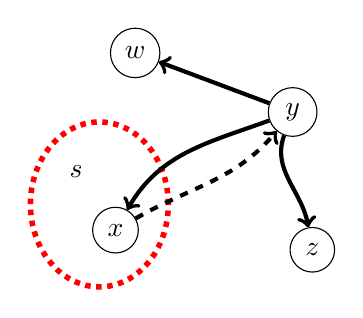
\begin{tikzpicture}[
			peer/.style={draw,shape=circle},
			query/.style={->,line width=1.5pt},
			resp/.style={->,line width=1.5pt,dashed}
			]
	\node[peer] (x) at (0, 0.25) {$x$};
	\node[peer] (w) at (0.25, 2.5) {$w$};
	\node[peer] (z) at (2.5, 0) {$z$};
	\node[peer] (y) at (2.25, 1.75) {$y$};

	\node (s) at (-0.5, 1) {$s$};

	\node[ellipse,draw=red,dotted,line width=2pt, fit=(s) (x)] {};

	\draw[query] (y) to (w);
	\draw[query,out=250,in=100] (y) to (z);

	\draw[query,out=200,in=60] (y) to (x);
	\draw[resp,out=30,in=230] (x) to (y);
	\end{tikzpicture}
}
\qquad
	\subfloat[Two responses]{
	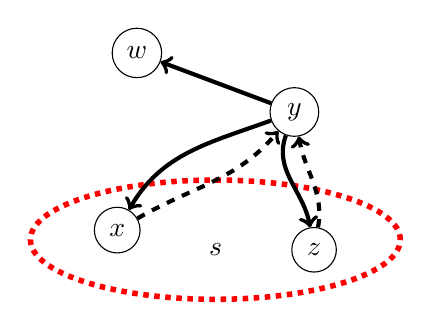
\begin{tikzpicture}[
			peer/.style={draw,shape=circle},
			query/.style={->,line width=1.5pt},
			resp/.style={->,line width=1.5pt,dashed}
			]
	\node[peer] (x) at (0, 0.25) {$x$};
	\node[peer] (w) at (0.25, 2.5) {$w$};
	\node[peer] (z) at (2.5, 0) {$z$};
	\node[peer] (y) at (2.25, 1.75) {$y$};

	\node (s) at (1.25, 0) {$s$};

		\node[ellipse,draw=red,dotted,line width=2pt, fit=(s) (x) (z)] {};

	\draw[query] (y) to (w);

	\draw[query,out=200,in=60] (y) to (x);
	\draw[resp,out=30,in=230] (x) to (y);

	\draw[query,out=250,in=100] (y) to (z);
	\draw[resp,out=80,in=280] (z) to (y);
	\end{tikzpicture}
}
	\caption{An attribution privacy leak. Black lines represent queries, dashed
	lines represent responses to a query. $y$ gains different amounts of
	information about the location of source $s$ depending on how many peers
	respond.}
	\label{fig:attack}
\end{figure}

To measure the attribution privacy risk in a P2P network, we start with the worst-case scenario. Suppose that for knowledge about some $q$
there is only a single source $s$, only a single peer $x$ with access to that
source (i.e. a single origin), and that $x$ has not shared any knowledge of $q$
with the rest of the network. Another peer $y$ who wants to learn about $K(q)$
might then query {\it every peer} in the network for knowledge about $q$. Since
$x$ has not previously shared information about $q$, every peer will respond
with no knowledge except for $x$.

$y$ now knows that of all the peers, only $x$ has knowledge about $q$. Because
the network is closed, $y$ also knows that there must be a source for $q$ among
the peers who know about $q$. Thus $x$ must possess a source for $q$ and since
we assumed there was only one such source, it must be $s$. Thus by sharing their
knowledge about $q$, $x$ has inadvertently shared the fact that they possess
source $s$. This is illustrated in \figref{attack}(a).


We can reason that this is the worst possible case as follows: if there were
multiple sources related to $q$, then $y$ would only know that $x$ possesses one
of those sources; it would not necessarily know which one. Also, if there were
multiple peers with access to a source for $q$, then multiple peers would
respond when $y$ queries every peer about $q$ (see \figref{attack}(b)). The same would occur if $x$ had
previously shared knowledge about $q$ with other peers in the network. In both
of these cases we can quantify the information gained by $y$. Let $S$ be the
event that one of the peers is an origin for $q$ (i.e. has
source $s$) and let $H$ be the number of peers who have the knowledge and thus
respond to the query.
If $k$ peers respond to the query, then we can express $P(S|H=k)$ in terms of
$P(S)$, the prior probability of a peer being an origin:
\begin{align}
	P(S|H=k)&=P(S|\text{one of the $k$ is a source})=\frac{P(S\cap\text{one of
	the $k$ is a source})}{P(\text{one of the $k$ is a source})}\nonumber\\
	&=\frac{P(S)}{1-P(\text{none of the $k$ are sources})}\label{eq:psksub}\\
	&=\frac{P(S)}{1-(1-P(S))^k}\label{eq:psk}
\end{align}
Note that we can simplify to \eqref{eq:psksub} because the event $S$ is included
in the event that one of the $k$ responders is a source. Note also that
$P(S|H=k)>P(S)$ for $P(S)\in(0,1)$. When $k=1$ (which is our previous assumption
that there is only one origin), $P(S|H=k)=1$ which agrees with our reasoning
that $y$ knows definitively that $x$ has source $s$. However if more than one peer
responds (either by multiple sources or by $x$ sharing knowledge), $y$ cannot be
certain whether $x$ has a source.

Going back to our original worst-case assumptions, suppose that after $y$
queries, another peer $z$ queries for information about $q$. Now we are in the
previously discussed weaker case: {\it two} peers will respond with knowledge
about $q$ ($x$ and $y$)! Thus $z$'s information about $s$ is only $P(S|H=2)<1$.

\begin{theorem}
	If $k$ peers in the network have knowledge of $q$, then
	\begin{equation*}
		P(S|\text{the peer responds to a query})\le P(S|H=k)
	\end{equation*}
\end{theorem}
\begin{proof}
	This follows from the definition in \eqnref{psk} and the previous arguments.
\end{proof}

The goal of a private attribution network is to make $P(S|\text{the peer
responds to a query})$ smaller than $P(S|H=k)$.

\subsection{Unreliable Peers}\label{sec:unreliable}

One simple approach to improving the privacy of the network is for the peers to
be unreliable i.e. let $P(\text{respond to a query about }q|\text{have knowledge
of }q)=r<1$. This is similar to the ``randomized response'' method of
differential privacy\cite{randresps}, but with the crucial difference that a peer
without knowledge of $q$ will never lie about it. Unlike differential
privacy---which provides privacy at the expense of introducing noise into the
data---we are interested in sharing only accurate data in the P2P network.

Now when $y$ queries the entire network, they can no longer be sure
that the peers who respond are all the peers who have the relevant knowledge.
Thus we now have a new random variable $M\ne H$ which is the number of peers who
respond to a query about $q$.

If $m$ peers respond to a query, in order to calculate the posterior, $y$ must
consider how many peers in the network actually have knowledge about $q$, which
can range from $m$ to $n-1$ (since $y$ does not know about $q$).
\begin{align}
	P(S|M=m)&=\sum_{k=m}^{n-1}P(S\cap H=k|M=m)\nonumber\\
	&=\sum_{k=m}^{n-1}\frac{P(S\cap H=k\cap M=m)}{P(M=m)}\frac{P(H=k\cap
	M=m)}{P(H=k\cap M=m)}\nonumber\\
	&=\sum_{k=m}^{n-1}P(S|H=k\cap M=m)P(H=k|M=m)\nonumber\\
	&=\sum_{k=m}^{n-1}P(S|H=k)\frac{P(M=m|H=k)P(H=k)}{P(M=m)}\label{eq:psmsimp}\\
	&=\frac{1}{P(M=m)}\sum_{k=m}^{n-1}P(S|H=k)P(M=m|H=k)P(H=k)\label{eq:psmbig}
\end{align}
where $P(S|H=k)$ is calculated as in \eqnref{psk} and we can simplify to
\eqref{eq:psmsimp} because $S$ is independent of $M$ if we know $H=k$.
We see that now the posterior probability of a source depends on the prior
distribution of knowledge in the network $H$. We also see the prior probability
of $M$, but this too can be expressed in terms of $H$:
\begin{align*}
	P(M=m)=\sum_{k=m}^{n-1}P(M=m\cap H=k)=\sum_{k=m}^{n-1}P(M=m|H=k)P(H=k)
\end{align*}

Lastly we observe that $P(M=m|H=k)$ is simply given by the binomial
distribution $b(m,k,r)$: the probability of $m$ successes out of $k$ trials where
each trial has probability $r$ of success. Substituting into \eqnref{psmbig} gives us
\begin{equation}\label{eq:psm}
	P(S|M=m)=\frac{\sum_{k=m}^{n-1}P(S|H=k)b(m,k,r)P(H=k)}{\sum_{k=m}^{n-1}b(m,k,r)P(H=k)}
\end{equation}

\begin{theorem}\label{th:rbound}
	$P(S|M=m)\le P(S|H=m)$ and this inequality is strict if $r<1$.
\end{theorem}
\begin{proof}
	Suppose that $r=1$, then $P(H=m)=1$ so \eqnref{psm} simplifies to
	\begin{equation*}
		P(S|M=m)=\frac{P(S|H=m)b(m,m,r)P(H=m)}{b(m,m,r)P(H=m)}=P(S|H=m)
	\end{equation*}
	Now suppose $r<1$, by \eqnref{psk} we have that
	\begin{equation*}
		P(S|H=k+1)=\frac{P(S)}{1-(1-P(S))^{k+1}}<\frac{P(S)}{1-(1-P(S))^k}=P(S|H=k)
	\end{equation*}
	therefore
	\begin{align*}
		P(S|M=m)&=\frac{\sum_{k=m}^{n-1}P(S|H=k)b(m,k,r)P(H=k)}{\sum_{k=m}^{n-1}b(m,k,r)P(H=k)}\\
		&<\frac{\sum_{k=m}^{n-1}P(S|H=m)b(m,k,r)P(H=k)}{\sum_{k=m}^{n-1}b(m,k,r)P(H=k)}\\
		&=P(S|H=m)\frac{\sum_{k=m}^{n-1}b(m,k,r)P(H=k)}{\sum_{k=m}^{n-1}b(m,k,r)P(H=k)}\\
		&=P(S|H=m)
	\end{align*}
\end{proof}

One concern with such a change to the P2P protocol is the potential performance
impact. Smaller $r$ will increase the overall number of queries which need to be
made in order for the knowledge to spread, thus decreasing the overall speed of
the network. This impact is measured empirically in \secref{qgiveni}.

\subsection{Extra Responses}\label{sec:exre}

Since $P(S|H=k)$ decreases as $k$ increases, another method of
preserving privacy would be for the peers responding to queries to force $k$ to
be large. Specifically, whenever a peer responds to a query it also
sends that response to each other peer with probability
$\frac{t}{n-2}$. Since there are $n-2$ peers other than $x$ and $y$, we expect
that $t$ extra responses will be sent.

Applying this change in protocol to our worst-case situation, we see that $y$
still knows with $P(S|H=1)=1$ that $x$ has source $s$. However, afterwards $x$,
$y$, and $t$ random peers are expected to know about $q$ thus the next peer
to make a query has an expected advantage of only $P(S|H=t+2)$. We can minimize this
probability by making $t$ even larger: $t=n-2$ means that $x$ sends extra
responses to every other peer, and then the next peer won't query at all because
every peer already has the data!

But this view is oversimplified. Although this does minimize the posterior
probability of $x$ having $s$ following a query, it just leaks the
information earlier in the process. For example, consider a swarm of just four
peers $x$, $y$, $\beta$, and $\gamma$ and suppose that $t=2$. $y$ starts as usual by
querying every peer about $q$ ($x$, $\beta$, and $\gamma$). Only $x$ has knowledge of
$q$, so it responds to $y$ and sends extra responses with probability
$t/(n-2)=1$ to peers $\beta$ and $\gamma$. From $\beta$'s perspective, since it received a
query about $q$ from $y$, it knows that $x$ and $\gamma$ were also queried. Since a
queried peer always sends extra responses if it has the knowledge, $\beta$ knows that
every peer who sends it an extra response knows about $q$. It received an extra
response only from $x$ thus it can apply the same logic as $y$ (in
\secref{baseline}) to deduce that $x$ has $s$.

Clearly, $t=n-2$ is too large. But even smaller values of $t$ leak some privacy to the
peers receiving extra responses. In fact, the situation generalizes to that of
\secref{unreliable}: when a query about $q$ is received by a peer $\beta$,
they expect to receive an extra response from each peer that has knowledge of
$q$ with probability $t/(n-2)$. It is as if $\beta$ itself made the query and each
peer responds probabilistically, which is exactly the situation with unreliable
peers, only now $r=t/(n-2)$ and $M$ is the number of extra responses received by
$\beta$.

% TODO diagram showing flooding attack

The point of sending out random extra responses would be defeated if
$P(S|M=m)>P(S|H=m)$ because then the extra responses a peer sends out would
actually leak more private information than if it were simply queried directly.
However we showed with \thref{rbound} that $P(S|M=m)<P(S|H=m)$ if $r<1$ i.e. if
$t<n-2$.
To choose $t$, we first note
a major difference from \secref{unreliable}: an attacker in this case
has some control over $r$ and thus $M$. If we have a swarm of $n$ peers,
an attacker can add $b$ malicious peers to the swarm. These malicious peers can
share information among themselves, such as who they have received extra
responses from. In effect, the $b$ peers behave like a single peer that has a
higher chance of receiving extra responses. We call this a ``flooding attack''.

\begin{theorem}
	If extra responses are sent with probability $\frac{t}{n-2}$, then the
	probability that an attacker inserting malicious peers into the network
	receives an extra response is bounded by $1-1/e^t$.
\end{theorem}
\begin{proof}
Let $B$ be the event that at least one of the $b$ malicious peers is sent an extra
	response and let $n$ be the original number of peers in the network. Then:
\begin{align*}
	P(B)&=1-P(\neg B)\\
	&=1-\left(1-P(\text{a particular malicious peer gets an extra response})\right)^b\\
	&=1-\left(1-\frac{t}{n+b-2}\right)^b\\
	\lim_{b\rightarrow\infty}P(B)&=1-\frac{1}{e^t}
\end{align*}
\end{proof}
Even for $t=5$ this probability is very close one, so we must choose a small $t$
if we consider such an attack to be viable.  Our only concern with small $t$
might be that it does not cause the knowledge to spread ``quickly enough'' to
provide a privacy benefit. However we will see in \secref{qgiveni} that even for
$t=1$ (which provides a limit of $1-1/e\approx2/3$), knowledge propagates very
quickly through the network.

Note that this leak also relies largely on the assumption that every peer
queries every other peer in order to greedily determine as much private
information as possible. In an actual P2P network, it is not necessary for each
peer to query every other peer. Thus with non-greedy peers, when a peer (or
group of malicious peers) is
{\it not} sent an extra response it is possible that it will also {\it not} receive the
corresponding query for $q$---in which case it will be completely oblivious to the
entire exchange and no leak will occur.

\section{Knowledge Distribution}\label{sec:kdist}

The privacy provided by both techniques from \secref{prrsk} depends on $P(H)$:
the prior probability distribution for the number of peers who possess knowledge
about some query $q$. In this section we will see that $P(H)$ is formulated in
much the same way as $P(S|M)$ from \secref{unreliable} and how the design of the
P2P protocol is crucial to its calculation.

Na\"ively, we could assume that at the time that we query for $q$, no other
peers have made similar queries. In that situation, the peers who
possess knowledge of $q$ would be exactly the set of origins: no queries have
been made, so no knowledge has spread beyond the sources for $q$. Then
\begin{equation*}
	P(H=k|\text{no queries})=P(k\text{ sources}|\text{at least one
	source})
\end{equation*}
since we need to assume sources exist in order to query for $q$. But this will
most likely not be accurate since queries have probably occurred between other
peers, thus changing the distribution of $H$.

However, assuming that our peers greedily query every other peer in the swarm
(in order to gain as much private knowledge as possible), we would know a priori
how many queries have been made for $q$. Thus our prior should really be
$P(H|Q)$ where $Q$ is the number of previously made queries for $q$. Even in the
non-greedy case where peers query some subset of the network, we could use the
number of observed queries to probabilistically calculate the prior.

% TODO link to future work about prob prior?

This prior can be formulated in much the same way as $P(S|M)$ from \eqnref{psm},
except instead of considering possible values of $H$ for $M$, we consider possible
values of $I$ for $Q$, where $I$ is the number of origins that were originally in the network:
\begin{align}
	P(H=k|Q=u)&=\sum_{i=1}^kP(H=k|I=i\cap Q=u)P(I=i|Q=u)\nonumber\\
	&=\frac{\sum_{i=1}^kP(H=k|I=i\cap
	Q=u)P(Q=u|I=i)P(I=i)}{\sum_{i=1}^{k}P(Q=u|I=i)P(I=i)}\label{eq:hgq}
\end{align}
All the terms in this formula can be calculated based on what we already know of
the network. $P(I=i)$, the prior probability of
there being $i$ origins, is simply given by $P(S)$ and the binomial
distribution: $P(I=i)=b(i,n-1,P(S))$. $P(H=k|I=i\cap Q=u)$, the probability of
$k$ peers knowing about $q$ after $i$ origins are queried $u$ times, can
be calculated based on the rate at which knowledge spreads through the network
(see \secref{hgiveniq}). $P(Q=u|I=i)$, the probability that $u$ queries are made
against $i$ origins, can also be calculated using the rate at which
knowledge spreads though from a different perspective (see \secref{qgiveni}).

\subsection{Conditional Knowledge Distribution}\label{sec:hgiveniq}

We showed previously how the distribution of knowledge given a certain number of
queries were made depends on the knowledge distribution also assuming the number
of origins: $P(H|I\cap Q)$.

The calculation of this distribution in effect measures how knowledge flows
through the network given a particular querying protocol. For example, given
the simple case where a peer simply responds to a query deterministically (as
in \secref{baseline}), we know that
\begin{equation*}
	P(H=i+u|I=i\cap Q=u)=1
\end{equation*}
because $i$ peers know initially and each of the $u$ queries passes on the
knowledge to one more peer.

If we have unreliable peers as in \secref{unreliable}, where a peer has
probability $r$ of responding to a query, we can easily calculate cases such as
\begin{align*}
	P(H=i|I=i\cap Q=1)&=(1-r)^i\\
	P(H=i+1|I=i\cap Q=1)&=1-(1-r)^i
\end{align*}
however the general calculation is far more complex as $Q$ increases (due to
multiple ways of achieving the same $H$). It takes the form
\begin{equation*}
	P(H=k|I=i\cap Q=u)=\sum_{\{F\}}\prod_{l=0}^{k-i-1}(1-r)^{(i+l)F_l}(1-(1-r)^{i+l})
\end{equation*}
where the sum is over all possible ways to have exactly $k-i$ successful queries
out of $u$ queries and the $F_l$ represent the number of failures before the
$l^\text{th}$ success. This could be efficiently calculated using dynamic
programming, however in practice we found that simulations of the
network to empirically calculate the probability converged reasonably quickly to
an accurate result (and are much simpler to implement). However we observe that
this calculation only appears in \eqnref{hgq} as a product with $P(Q=u|I=i)$. We
will see in \secref{qgiveni} that $P(Q=u|I=i)$ will only be nonzero for a
limited range of $i$. Thus in practice we need only calculate $P(H=k|I=i\cap
Q=u)$ when this product has a chance of being nonzero. See \secref{eval} for the
result.

Similarly for the case of extra responses from \secref{exre}, the general
probability calculation is surprisingly complex; one must consider which peers
were chosen to receive extra responses and how these peers overlap with each
other and the queried peers. Once again we chose to empirically calculate the
distribution via simulation.

\subsection{Query Distribution}\label{sec:qgiveni}

The second distribution which must be calculated is $P(Q|I)$, the probability of
observing a certain number of queries given a number of initial origins. We
calculate this by taking into account $\Omega$, the number of total queries
about $q$ that will be performed. Since we assume that every peer will
eventually want to learn about $q$, this is equivalent to measuring how many
queries it takes for every peer to have the knowledge.
\begin{equation}\label{eq:pqi}
	P(Q=u|I=i)=\sum_{v=0}^\infty P(Q=u\cap\Omega=v|I=i)
\end{equation}

With deterministic responses as in \secref{baseline}, if a peer were to
observe the network over its lifetime, given $i$ origins it would see $n-i-1$
queries: one for each of the peers that does not have the knowledge (not
counting itself). For this protocol, \eqnref{pqi} simplifies to
\begin{equation}\label{eq:pqisimple}
	P(Q=u|I=i)=P(Q=u\cap\Omega=n-i-1|I=i)=\frac{1}{n-i-1}
\end{equation}
for $u\in[1,n-i-1]$. The first equality follows from the fact that there must be
$n-i-1$ queries. The second follows because a priori we can only assume that
each of the $n-i-1$ peers is indistinguishable with respect to wanting knowledge
about $q$, thus each query must be equally likely.

As in the previous section, the calculations are more elaborate as we change the
protocol. For unreliable peers, $P(\Omega|I)$ is similar to a negative binomial
distribution (the number of trials needed to get a certain number of successes
in a Bernoulli process) however it is more complicated because the probability
of a query succeeding increases as more queries succeed. Once again we found it
more practical to simply empirically calculate $P(\Omega|I)$ via network
simulation and then use the same assumption of equally likely queries from
\eqnref{pqisimple} to get $P(Q|I)$.

% TODO change all n to 100 for final submission

\begin{figure}%
    \centering
	\subfloat[$P(\Omega|I)$]{{\includegraphics[width=0.5\textwidth]{chart_omega_unrel_100_20.pdf}}}%
	\subfloat[$P(Q|I)$]{{\includegraphics[width=0.5\textwidth]{chart_qdist_unrel_100_20.pdf}}}%
	\caption{Calculating $P(Q|I)$ with unreliable peers ($r=0.2$) via network
	simulation ($n=100$). Each line in (a) shows the distribution
	$P(\Omega|I=i)$ for different $i$, while lines in (b) show $P(Q|I=i)$.}
    \label{fig:unrelqueries}%
\end{figure}

\Figref{unrelqueries} shows the result of
calculating $P(\Omega|I)$ and $P(Q|I)$ in this manner for a fixed chance $r$ of
a peer responding. Note that as the number of origins increases, the probability
of a query succeeding approaches 1, thus $P(\Omega=n-i|I=i)\rightarrow 1$,
consequently $P(Q|I)$ approaches a uniform distribution (since this is similar
to the deterministic case of \eqnref{pqisimple}). A convenient byproduct of this
calculation is that we also see the performance impact of the protocol.
Because $P(\Omega|I)$ is also a sort of measure of how long it takes every peer
to learn the knowledge, it is a decent measure of the worst-case performance of
the network. We can see that for a small number of origins, while the smaller
values of $Q$ have the highest probabilities, $P(Q|I)$ has a long tail,
indicating that in some cases we might require significantly more queries
overall before the knowledge spreads.

\begin{figure}%
    \centering
	\subfloat[$P(\Omega|I)$]{{\includegraphics[width=0.5\textwidth]{chart_omega_exre_100_1.pdf}}}%
	\subfloat[$P(Q|I)$]{{\includegraphics[width=0.5\textwidth]{chart_qdist_exre_100_1.pdf}}}%
	\caption{Calculating $P(Q|I)$ with extra responses ($t=1$) via network
	simulation ($n=100$). The format is the same as \figref{unrelqueries}, but
	note the difference in scale for $\Omega$ and $Q$.}
    \label{fig:exrequeries}%
\end{figure}

We can use the same technique with a different simulation to find $P(Q|I)$ for
the case of extra responses. \Figref{exrequeries} shows this result for a fixed $t$.
This converges to a uniform distribution more slowly than unreliable peers does,
but note that the scale for $Q$ is much smaller: even for 1 origin, it is
unlikely to take more than 14 queries for the knowledge to spread completely.
This is because each successful query only slightly increases the chance of each
extra response being sent, but overall the number of extra responses causes the
knowledge to spread throughout the network at an exponential rate. This
alleviates our concern of using small $t$ that we had from \secref{exre}.

\begin{figure}%
    \centering
	\subfloat[$P(\Omega|I)$]{{\includegraphics[width=0.5\textwidth]{chart_omega_unexre_100_1_20.pdf}}}%
	\subfloat[$P(Q|I)$]{{\includegraphics[width=0.5\textwidth]{chart_qdist_unexre_100_1_20.pdf}}}%
	\caption{Calculating $P(Q|I)$ with unreliable peers and extra responses
	($r=0.2$, $t=1$) via network simulation ($n=100$). The format is the same
	as \figref{unrelqueries}, but note the difference in scale for $\Omega$ and
	$Q$.}
    \label{fig:unexrequeries}%
\end{figure}

Because these calculations are done empirically, it is straightforward to extend this to
the combination of the two techniques: unreliable peers where each peer sends
extra responses. The result is shown in \figref{unexrequeries}. As we might expect, the
resulting distribution exhibits a mix of those from figures
\ref{fig:unrelqueries} and \ref{fig:exrequeries}: slow convergence to a uniform
distribution with a moderately long tail. We observe in \secref{eval} that this
also translates to good privacy performance.

\section{Evaluation}\label{sec:eval}

With the calculations developed in the previous sections, we can finally
implement a private attribution network using the protocol changes from sections
\ref{sec:unreliable} and \ref{sec:exre} and measure the resulting private
knowledge leakage. We must do so empirically because of the empirical
calculations in \secref{kdist}.

\begin{figure}%
    \centering
	\includegraphics[width=0.75\textwidth]{chart_comp_unrel.pdf}
	\caption{Comparison of the unreliable peers protocol with varying $r$
	($n=100$). Each line represents the private leakage as a function of when
	the attacker queries (ignoring failed queries). E.g. the first point
	represents the leakage if an attacker is the first peer to make a successful
	query, the second point is if they are the second peer, etc. The leakage is
	averaged over thousands of network simulations, so it is possible for the
	actual leakage to be higher or lower in a specific situation. Note the
	logarithmic scale on the $X$ axis.}
    \label{fig:compunrel}%
\end{figure}

We chose to evaluate the worst case scenario (similar to \secref{baseline}): a
single query $q$ with a single source $s$ possessed by a single peer $x$. Then
for multiple iterations we simulated knowledge of $q$ spreading through the
network query-by-query, recording after each query the private information leak
in terms of $P(S|\text{$x$ responds to a query})$.

Our first question was about the effect of differing $r$ on the unreliable peers
protocol. The results of these measurements are shown in \figref{compunrel}.
The ``Worst case'' line is the leakage in the simple deterministic case from
\secref{baseline} where the leakage is simply given by $P(S|H=k)$. Note that
this is equivalent to the unreliable peers protocol with $r=1$. Because the
leakage of unreliable peers is given by $P(S|M=m)$, this figure
indicates that $P(S|M=m)$ converges to $P(S|H=k)$ as $m$ and $k$ increase and
that decreasing $r$ delays this convergence. For example, $r=0.8$ provides a
slight privacy benefit to only the first peer that is queried because it is nearly identical
by the second peer, whereas $r=0.2$ provides a privacy benefit to the first
three or four peers. Because the worst-case leakage approaches $P(S)$, we can
choose a point at which we deem this leakage negligible and choose $r$ such that
the convergence occurs after this point.

% TODO think about how P(S|M) can actually be greater than P(S|K) when m != k

\begin{figure}%
    \centering
	\includegraphics[width=0.75\textwidth]{chart_comp.pdf}
	\caption{Comparison of different network protocols ($n=100$, $r=0.2$, $t=1$).
	The format is the same as in \figref{compunrel}.}
    \label{fig:comp}%
\end{figure}

Next we compared the effect of the different protocols, shown in \figref{comp}.
As expected, extra responses provides no privacy benefit if the attacker is the
first peer to query, since the intention is to provide higher privacy to {\it
later} queries. Indeed the leakage decreases more quickly for extra
responses than it does for unreliable peers, beating it by the third or fourth
query. By the tenth or so query, the leakage is already negligible compared to
$P(S)$. By that point it is likely that almost every peer has the knowledge,
thus $k\approx n$ and $P(S|H=k)\approx P(S)$.

``Both'' shows the effect of combining both unreliable peers and extra
responses. The resulting protocol provides a good balance between the two: it
has a low initial leakage for the first few peers to be queried, but also
approaches $P(S)$ much quicker than the worst case. We were surprised to see
that the leakage was even lower than unreliable peers with the same $r$.
Although we are uncertain of the exact reason for this, we speculate that this
is due to the $P(S|M)$ calculation involving $P(H)$ (\eqnref{psm},
\secref{unreliable}). The extra responses
shrink $P(H=k)$ for small $k$ (because the knowledge spreads quicker), thus a
small number of peers responding to a query are likely to be part of a larger
set of peers who actually have the knowledge, which results in smaller $P(S|M)$.

\begin{figure}%
    \centering
	\includegraphics[width=0.75\textwidth]{chart_exre_dist_100_1.pdf}
	\caption{Distribution of privacy leakage due to extra responses. The black
	curve is identical to the extra responses curve in \figref{comp} (though
	mirrored). The perpendicular curves show the distribution of leakage among
	all other peers in the network, resulting from extra responses sent during
	that attacker's query.}
    \label{fig:exdist}%
\end{figure}

\begin{figure}%
    \centering
	\includegraphics[width=0.75\textwidth]{chart_unexre_dist_100_1_20.pdf}
	\caption{Distribution of privacy leakage due to extra responses with
	unreliable peers. The format is the same as in \figref{exdist}.}
    \label{fig:uexdist}%
\end{figure}

\Figref{comp} is slightly misleading because the two protocols involving extra
responses only provide a faster leakage falloff because the extra responses
spread out the leakage more uniformly in the network. Thus we need to measure
the distribution of this leakage in order to determine if the trade-off is worth
it. The results are shown in figures \ref{fig:exdist} and \ref{fig:uexdist}. We
can see that for early queries, this leakage is insignificant as we would expect:
few peers are likely to receive an extra response at all. For later queries,
the leakage becomes more uniform as the number of extra responses increases,
however we see that significant leakage never extends beyond around 30\% of the
network ($n=100$), and even then the leakage is already so close to $P(S)$ that
it could be considered acceptable.

\section{Discussion \& Conclusion}

We have shown that although attribution privacy can be a significant risk in
certain situations, the techniques we have developed in this paper can be
employed to effectively mitigate the risk. The method of unreliable peers can be
applied (with a carefully chosen parameter) to ensure that a desired level of
privacy is maintained even when a small number of peers respond to a query.
The method of extra responses can be applied to ``pay
forward'' privacy to other peers in the network by ensuring the knowledge
spreads faster. Although extra responses make the network susceptible to an
attacker that floods the network with malicious peers, the risk can be
controlled by carefully choosing the parameter for the extra responses.
Furthermore, we showed empirically that these two methods synergize to provide
an even greater privacy benefit than either method on its own.

We conclude that the methods of unreliable peers and extra responses are a firm
starting point for any P2P application in which attribution privacy is involved.
They can be tuned to preserve (or increase) network performance while
maintaining whatever level of privacy is demanded by the application.

\subsection{Future Work}\label{sec:future}

As mentioned in \secref{relwork}, this research was originally part of a much
larger project, and there still remain several barriers preventing a practical
implementation of a private attribution network. First, we were only able to
measure network performance in terms of the maximum number of queries needed for
knowledge of a single query to fully spread. It is unclear what exactly the
affect would be on an individual level, for a peer making many separate queries
with different sources. We also assumed that every peer queries every other
peer, as this simplified analysis and also matched the behavior that an attacker
might use in order to learn as much private information as possible. But in a
practical implementation, this behavior may not be desirable (for non-malicious
peers). It would be interesting to see what the ``accidental'' leakage is if
peers query only a subset of the network, and how this leakage is affected by
the two protocols we examined. Both the performance and accidental leakage
depend greatly on the specific use-case of the private attribution network, so
we leave their investigation to future researchers.

We also considered a mechanism similar to extra responses, where a peer would
actually not reply to the querying peer at all. Instead the peers receiving
extra responses would be responsible for eventually relaying the data back to
the peer that made the query. This would provide even greater privacy by masking
the replying peer from the querying peer in a Tor-like way, while also spreading
knowledge through the network via the extra responses. Unfortunately we were
unable to quantify the privacy provided by this method during our research. This
could also be extended as a method for peers to gain knowledge without needing
to query the entire network, by having the queried peers send out {\it extra
queries} on behalf of the original querying peer.

One potential attack that we did not have time to address is if an attacker
makes repeated queries in order to circumvent the randomness of the unreliable
peers protocol. Such an attack could be implemented similar to the flooding
attack of extra responses, where multiple malicious peers all make the same
query and collaborate to artificially increase $r$. This could be defended
against by choosing $r$ inversely proportional to $n$ as with extra responses,
or by regulating responses such that an unreliable peer will consistently lie
about a query for some time after initially queried.

We described attribution privacy in an asymmetric setting where an attacker
queries a potentially vulnerable peer. But this could also be extended to a
situation where the queries themselves are sensitive. In our Nickelback example
from \secref{nickelback}, we can imagine that someone might be equally
embarrassed to ask about a Nickelback song, for fear of appearing to be a
Nickelback fan themselves. Or in the advertisement example from \secref{xray},
someone querying about an ad might reveal that they possess the sensitive data
which the ad targets. In such cases, the P2P network would need to protect both
the querying peer and the queried peer.

\begin{thebibliography}{9}

\bibitem{privatep2p}
	M. Rogers, S. Bhatti.
	How to Disappear Completely: A Survey of Private Peer-to-Peer Networks.
	\emph{Sustaining Privacy in Autonomous Collaborative Environments (SPACE)}, 2007.

\bibitem{xray}
	M. L\'ecuyer, G. Ducoffe, F. Lan, A. Papancea, T. Petsios, R. Spahn, A. Chaintreau, and R. Geambasu.
	XRay: Enhancing the Web's Transparency with Differential Correlation.
	\emph{USENIX Security}, 2014.

\bibitem{chord}
	I. Stoica, R. Morris, D. Karger, M.F. Kaashoek, H. Balakrishnan.
	Chord: A Scalable Peer-to-peer Lookup Service for {Internet} Applications.
	\emph{Proceedings of the {ACM} {SIGCOMM} '01 Conference}, Aug 2001.

\bibitem{randresps}
	C. Dwork, A. Roth.
	The Algorithmic Foundations of Differential Privacy.
	\emph{Foundations and Trends in Theoretical Computer Science} 9.3-4 (2014): 211-407.

\end{thebibliography}

\end{document}
